\section{Efectul fotoelectric extern}

\subsection{Legile efectului fotoelectric extern}

\emph{Efectul fotoelectric} reprezintă emisia de electroni, numiți
fotoelectroni, de către o substanță sub acțiunea radiației electromagnetice.

Heinrich Hertz a descoperit acest fenomen în 1887, după ce a constatat că
o descărcare electrică se produce mai ușor atunci când electrozii sunt iluminați
de un arc electric, decât atunci când descărcarea se producea în întuneric.

\clearpage

\begin{wrapfigure}{r}{0.4\textwidth}
    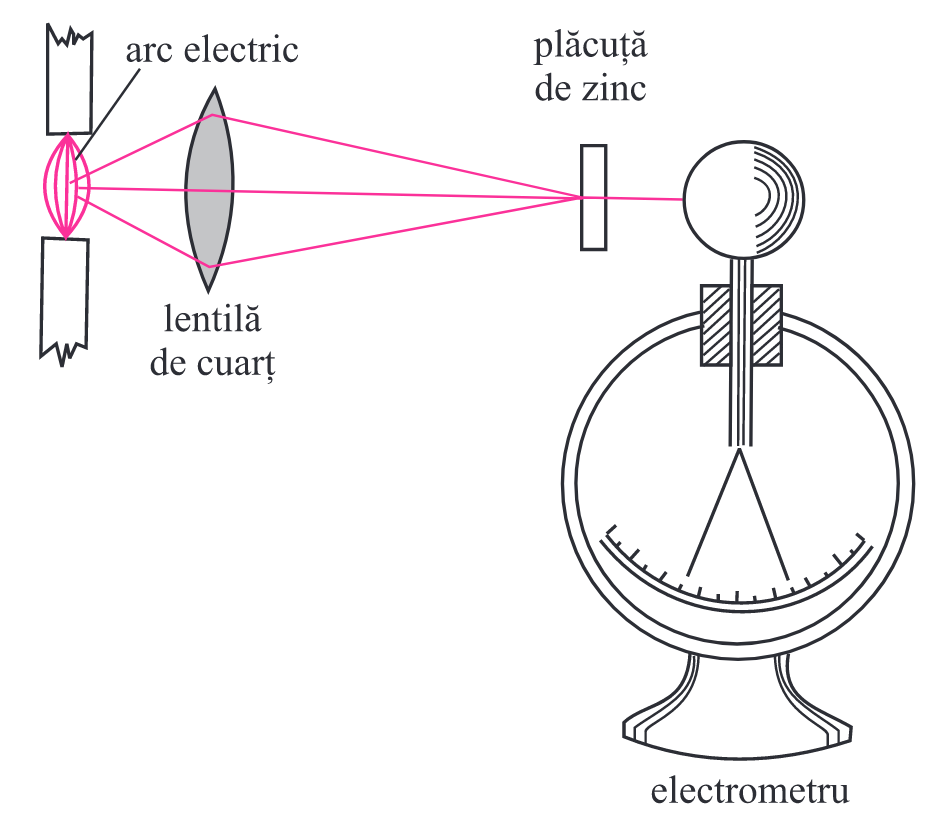
\includegraphics[width=0.35\textwidth]{fig/hallwachs}
    \caption{Schema experienței lui Hallwachs}
\end{wrapfigure}

Fizicianul englez Wilhelm Hallwachs a observat apoi în 1888 că, atunci când
focaliza radiația pe o placă de zinc încărcată electric negativ, folosind o
lentilă de cuarț, radiațiile ultraviolete conținute în arcul electric ce cădeau
pe placă cauzau pierderea sarcinii electrice a acesteia. În schimb, acest
fenomen nu avea loc dacă înlocuia lentila de cuarț cu una de sticlă, care
absorbea radiația ultravioletă. Repetând experiența pentru diferite stări
de încărcare a plăcii de zinc, observând deviațiile foițelor de aur ale
electrometrului, Hallwachs a concluzionat că, sub acțiunea radiațiilor
ultraviolete, placa de zinc emite particule încărcate negativ, denumite
ulterior electroni.

\begin{wrapfigure}{l}{0.4\textwidth}
    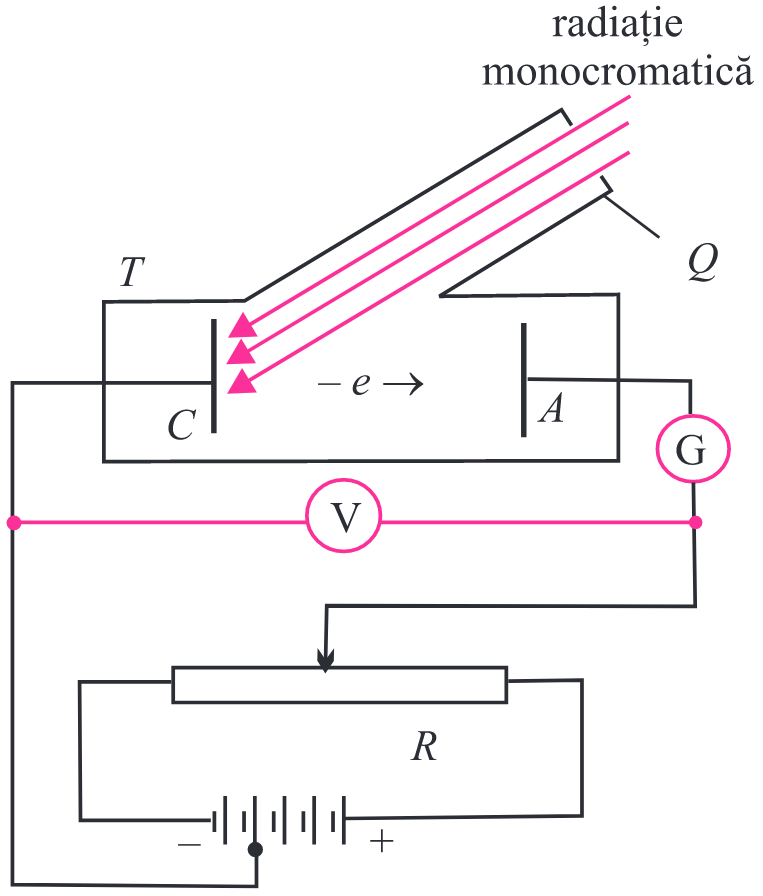
\includegraphics[width=0.35\textwidth]{fig/dispozitiv}
    \caption{Schema dispozitivului pentru studiul efectului fotoelectric extern}
    \vspace{1cm}
    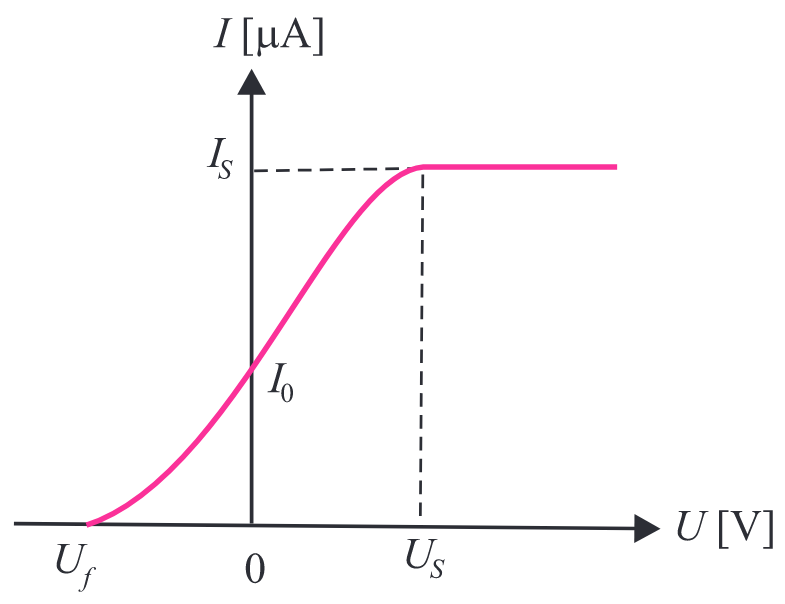
\includegraphics[width=0.35\textwidth]{fig/graph_I_fU}
    \caption{Dependența \( I = f(U) \) a efectului fotoelectric}
\end{wrapfigure}

Pentru a studia efectul fotoelectric extern se utilizează un dispozitiv format
dintr-un tub de sticlă vidat ($T$), prevăzut cu o fereastră de cuarț ($Q$), și
doi electrozi interiori, catodul ($C$) și anodul ($A$). Prin fereastra $Q$,
transparentă pentru radiațiile ultraviolete, se realizează iluminarea catodului
fotoelectrono-emisiv.

Electrozii catod și anod sunt conectați la o sursă de curent continuu, prin
intermediul unui montaj potențiometric, folosind reostatul $R$.

Pentru determinarea relației curent-tensiune \( I = f(U) \) a dispozitivului,
se folosesc voltmetrul $V$ și microampermetrul (galvanometrul) $G$.

Menținând constante frecvența $\nu$ și fluxul radiației electromagnetice $\Phi$
care cade pe catod, din studiul caracteristicii curent-tensiune (fig. 3) putem
observa următoarele proprietăți ale fenomenului:

\begin{itemize}
    \item Pentru valori $U$ mai mari decât o anumite tensiune $U_s$, intensitatea
        curentului atinge o anumită valoare maximă (de saturație) $I_s$.
    \item La anularea tensiunii, intensitatea curentului este nenulă ($I_0$).
    \item Pentru anularea intensității curentului, este necesară aplicarea unei
        tensiuni inverse $U_f$, numită \emph{tensiune de frânare}.
\end{itemize}

\clearpage

Între tensiunea de frânare $U_f$ și energia cinetică maximă a fotoelectronilor
emiși $E_{cM}$ există relația:
\[ E_{cM} = eU_f \]
unde $e$ este sarcina electronului.

Modificând fluxul și frecvența radiației electromagnetice, obținem legile efectului
fotoelectric extern:

{%
    \begin{minipage}{0.55\textwidth}
        \renewcommand{\labelenumi}{\textbf{\Roman{enumi}.}}
        \begin{enumerate}
            \item Intensitatea curentului fotoelectric de saturație $I_s$ este
                direct proporțională cu fluxul $\Phi$ al radiațiilor
                electromagnetice incidente, când frecvența $\nu$ este constantă
                (fig. 4).
            \item Energia cinetică maximă $E_{cM}$ a fotoelectronilor este
                proporțională cu frecvența radiației incidente, și nu depinde de
                fluxul acesteia (fig 5).
            \item Efectul fotoelectric extern se produce doar pentru radiații
                incidente cu frecvența mai mare decât o anumită frecvență de prag
                $\nu_0$, care este caracteristică a fiecărui metal în parte (fig 6). \\
                Metalele au frecvențe de prag în domeniul vizibil și în ultra-violet.
            \item Efectul fotoelectric se produce practic instantaneu, intervalul
                de timp dintre căderea radiației incidente și emisia fotoelectronilor
                fiind de ordinul $10^{-10}$ s.
        \end{enumerate}
    \end{minipage}%
    \hspace{0.5cm}%
    \begin{minipage}{0.35\textwidth}
        \centering
        \captionsetup{type=figure}
        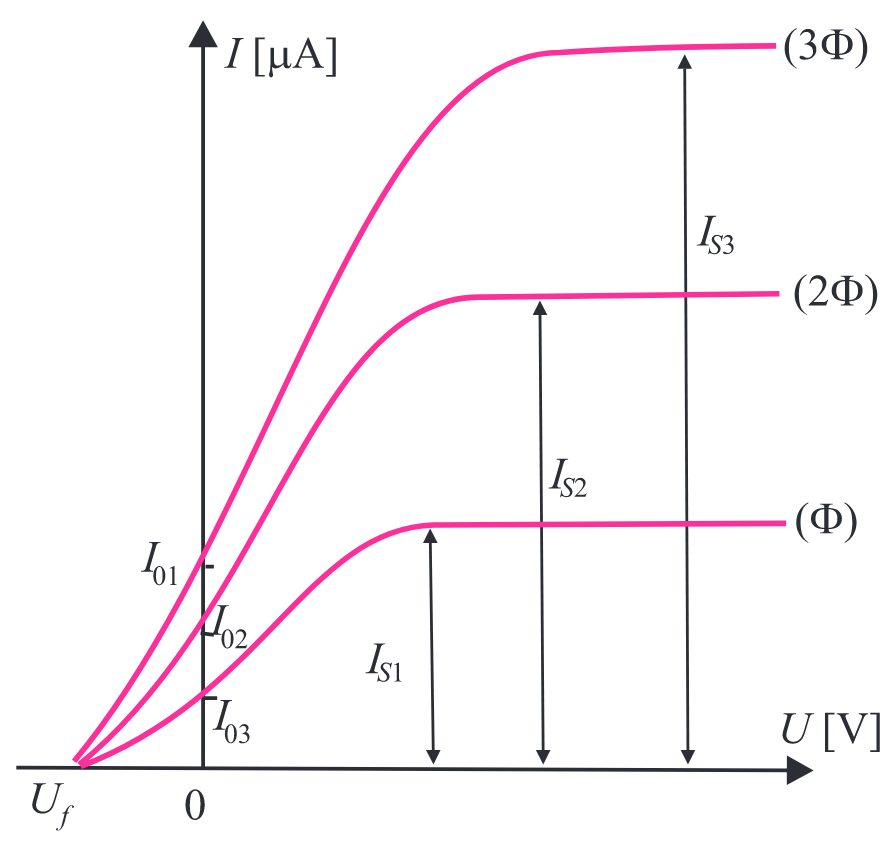
\includegraphics[width=\textwidth]{fig/graph_legea_1.png}
        \captionof{figure}{Ilustrarea primei legi a efectului fotoelectric extern}

        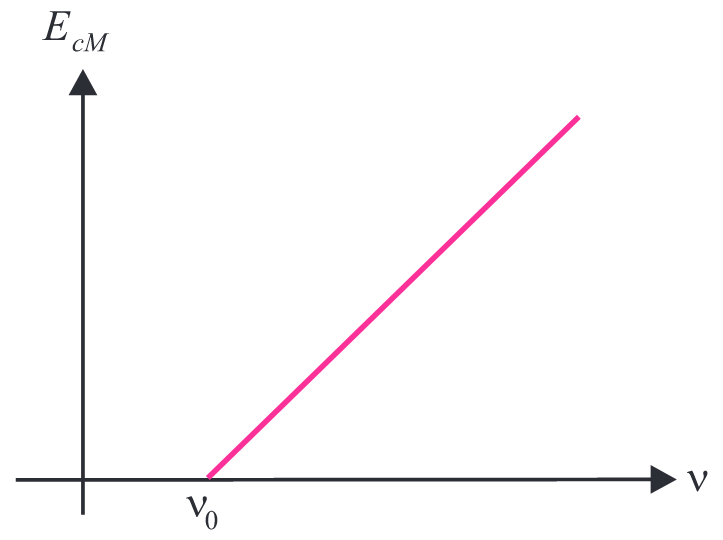
\includegraphics[width=\textwidth]{fig/graph_legea_2.png}
        \captionof{figure}{Dependența liniară a energiei cinetice maxime a fotoelectronilor de frecvența radiației incidente}

        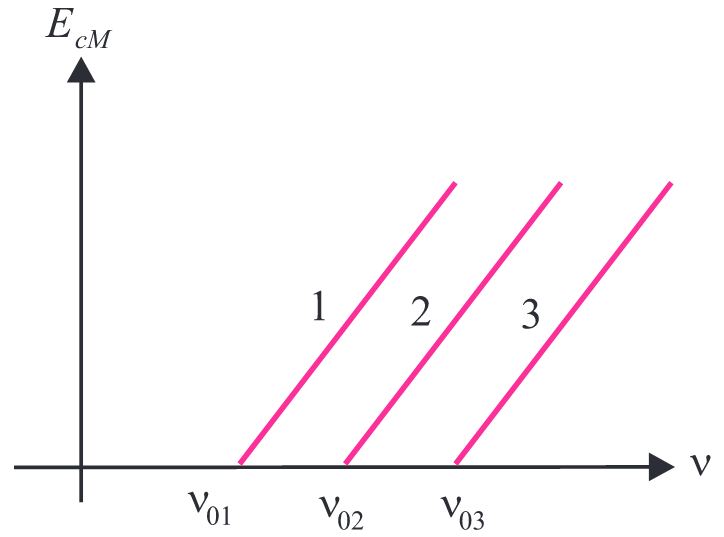
\includegraphics[width=\textwidth]{fig/graph_legea_3.png}
        \captionof{figure}{Dependența liniară a energiei cinetice maxime a fotoelectronilor de frecvența radiațiilor incidente pentru fotocatozi diferiți}
    \end{minipage}
}

\parbreak

\emph{Lucrul de extracție} $L_e$ este o mărime caracteristică fiecărui metal,
și reprezintă lucrul mecanic necesar pentru extragerea unui electron de pe
suprafața acelui metal. Valorile sale sunt cuprinse între $0,5$ și $5$ eV.


\subsection{Interpretarea legilor efectului fotoelectric extern}

Legile efectului fotoelectric extern, stabilite pe cale experimentală, nu pot fi
explicate cu ajutorul teoriei ondulatorii. Ajungem astfel la anumite neconcordanțe:

\begin{itemize}
    \item Din figura 4, observăm că tensiunea de frânare are aceeași valoare,
        indiferent de valoarea fluxului de energie luminoasă $\Phi$ care cade
        pe catod. Înseamnă că energia cinetică a electronilor emiși nu crește,
        deci nu depinde de flux.

        Conform teoriei ondulatorii, unda electromagnetică ce interacționează
        cu substanța ar trebui să producă oscilații forțate ale electronilor
        din compunerea acesteia. Valoarea fluxului, energia undei, și pătratul
        amplitudinii sunt proporționale \( (\Phi \sim E_t \sim A^2) \),
        deci energia electronilor extrași ar trebui să fie proporțională cu
        amplitudinea undei incidente, și deci cu fluxul, ceea ce se află în
        neconcordanță cu legea a II-a.

    \item Legea a III-a afirmă că efectul fotoelectric se produce numai pentru
        o anumită frecvență de prag, însă conform teoriei ondulatorii fenomenul
        ar trebui să aibă loc pentru orice frecvență a radiațiilor incidente,
        dacă intensitatea lor este suficient de mare.

    \item Legea a IV-a stabilește că efectul fotoelectric are loc practic
        instantaneu, însă conform teoriei ondulatorii, între momentul punerii
        în oscilație forțată a electronilor și momentul emisiei (adică până
        când electronii preiau energia necesară), ar trebui să se scurgă un
        anumit interval de timp (aproximativ 4000 s).
\end{itemize}

\subsection{Ipoteza lui Planck. Ipoteza lui Einstein. Ecuația lui Einstein}

Teoria cuantelor, elaborată în 1900 de către Max Planck (Premiul Nobel în
1918), permite corecta interpretare a legilor efectului fotoelectric extern.
Planck a emis ipoteza, confirmată ulterior, că \emph{schimbul de energie între
microsistemele fizice (atomi, molecule, ioni, nucleu) prin intermediul
radiației electromagnetice nu se realizează continuu, ci discret, energia
schimbată fiind cuantificată în porții $h\nu$}, unde $\nu$ este frecvența
undei, iar \( h = 6,626075 \cdot 10^{-34} ~ \mathrm{J \cdot s} \) este
constanta lui Planck, constantă fizică universală, ce apare în fenomenele
fizice la scară microscopică.

În 1905, Einstein a presupus că radiația electromagnetică cu frecvența $\nu$
este alcătuită dintr-o mulțime de particule, denumite ulterior fotoni, fiecare
având energia \( E_f = h\nu \). Atunci când părăsește metalul, electronul va
avea o anumită energie cinetică. Bilanțul energetic conduce la
\emph{ecuația lui Einstein}:
\[ h\nu = L_e + E_{cM} \]

S-a considerat energia cinetică maximă deoarece $L_e$ reprezintă lucrul mecanic
de extracție a unui electron de pe suprafața metalului. Pentru electronii
aflați pe straturi interioare din metal, lucrul de extracție este mai mare
($L > L_e$), deci energia cinetică a fotoelectronilor este mai mică decât
$E_{cM}$. În acest caz, ecuația se scrie sub forma:
\[ h\nu = L + \frac{m_e v^2}{2} \]

Cum \( eU_f = E_{cM} \), ecuația lui Einstein se mai poate scrie și sub forma:
\[ h\nu = L_e + eU_f \]

Lumina este formată dintr-un ansamblu de fotoni, care, ca orice particule, au
energie și impuls.

Cunoscând relația dintre energie și masă în teoria relativității, \( E = mc^2 \),
și \( E = h\nu \), rezultă \( h\nu = mc^2 \), și obținem \emph{masa de mișcare} a
fotonului:
\[ m = \frac{h\nu}{c^2} \]

Viteza fotonului este egală cu viteza luminii, \( v = c \). Din formula relativistă
\( m = \frac{m_0}{\lorentzradical} \) rezultă că masa de repaus a fotonului este egală cu zero:
\[ m_0 = m\lorentzradical = 0 \]

Impulsul este:
\[ p = mc = \frac{h\nu}{c} = \frac{h}{\lambda} \]

\parbreak

Așadar, mărimile fizice ale fotonului sunt:
\begin{itemize}
    \newcommand{\boxlabel}[1]{\makebox[4cm][l]{#1}}
    \item \boxlabel{energia} $h\nu$
    \item \boxlabel{viteza} $v = c$
    \item \boxlabel{masa de mișcare} \( m = \frac{h\nu}{c^2} \)
    \item \boxlabel{masa de repaus} $m_0 = 0$
    \item \boxlabel{impulsul} \( p = \frac{h\nu}{c} = \frac{h}{\lambda} \)
\end{itemize}

\parbreak

Explicațiile legilor efectului fotoelectric extern în fizica cuantică sunt
următoarele:
\begin{enumerate}
    \renewcommand{\labelenumi}{\textbf{\Roman{enumi}.}}
    \item Legea I poate fi explicată atât prin teoria ondulatorie, cât și cu ajutorul
        fizicii cuantice.

        Valoarea de saturație a curentului este atinsă atunci când toți
        electronii emiși de catod în unitatea de timp sunt captați de anod. Cu
        cât fluxul radiației incidente este mai mare, numărul fotonilor
        incidenți este mai mare.  Deci numărul electronilor crește, ceea ce
        duce la creșterea valorii intensității de saturare.

    \item Din relația \( h\nu = L_e + E_{cM} \) rezultă că energia cinetică maximă
        a electronilor a fotoelectronilor emiși este:
        \[ E_{cM} = h\nu - L_e \]
        Relația evidențiază variația liniară a energiei cinetice a electronilor emiși
        cu frecvența, după cum rezultă și din legea a II-a.
    \item Pentru o anumită valoare a frecvenței, $E_{cM}$ devine nulă, obținându-se:
        \[ L_e = h\nu_0 \]
        În acest caz energia absorbită de la foton este folosită doar pentru a extrage
        fotoelectronul, după cum afirmă legea a III-a. La frecvențele mai mici decât
        frecvența de prag $\nu_0$, efectul fotoelectric extern nu mai apare.
    \item Interacțiunea dintre un foton și electron se produce într-un interval
        de timp neglijabil, așadar efectul fotoelectric extern se produce aproape
        instantaneu, după cum afirmă legea a IV-a.
\end{enumerate}

\parbreak

În concluzie, ipoteza privind caracterul corpuscular al radiației electromagnetice
explică legile efectului fotoelectric extern. Pe de altă parte, teoria ondulatorie a
undelor electromagnetice trebuie menținută, deoarece legile clasice sunt valabile în
privința propagării câmpului electromagnetic (difracția, interferența). Aceste două
caracteristici diferite pot fi corelate, după cum se va arăta ulterior.

\subsection{Aplicații ale dispozitivelor optoelectronice}

Efectul fotoelectric extern stă la baza funcționării celulei fotoelectrice,
care produce semnale electrice prin iluminare. Este folosită, de exemplu, la
releul fotoelectric, la redarea sunetelor în cinematograful sonor, în
televiziune, pentru transformarea semnalelor luminoase în semnale electrice.

\begin{wrapfigure}{r}{0.6\textwidth}
    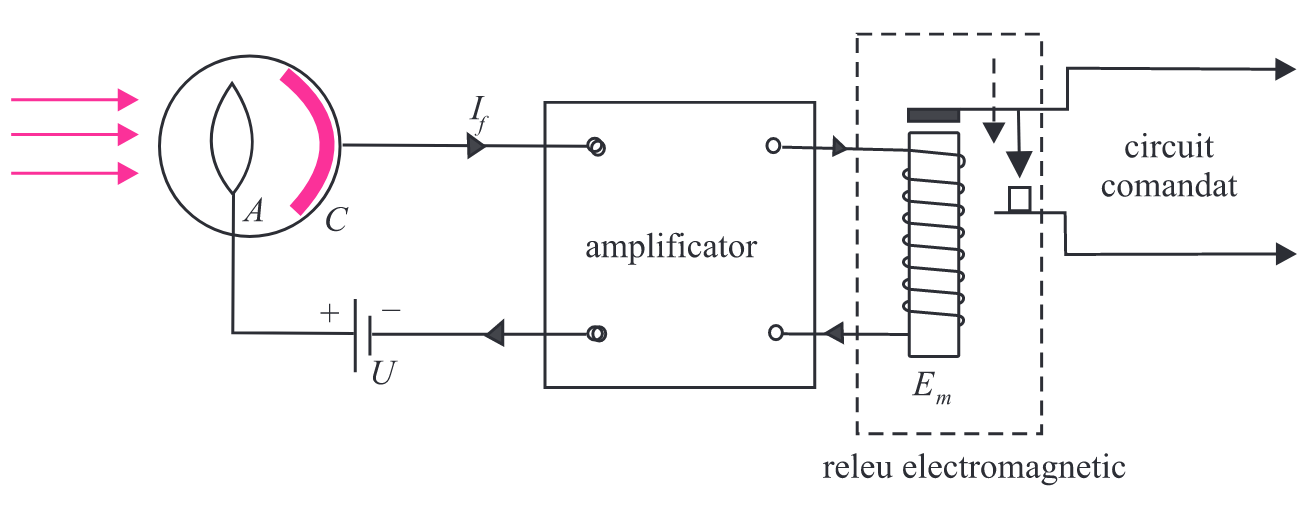
\includegraphics[width=0.6\textwidth]{fig/releu_fotoelectric}
    \caption{Releul fotoelectric}
\end{wrapfigure}

Releul fotoelectric este un releu electromagnetic comandat de o celulă
fotoelectrică (fig. 7). Lumina cade pe fotocatod, determinând apariția unui
fotocurent de intensitate $I_f$ care, după amplificare, trece prin circuitul
unui electromagnet $E_m$, al cărui câmp magnetic provoacă închiderea circuitului
comandat.

Deoarece comanda este sigură, rapidă, practic fără inerție, releul fotoelectric
este folosit pentru numărarea unor corpuri în mișcare, pentru semnalizarea
prezenței umane, pentru conectarea automată a rețelei de iluminat când se
întunecă, pentru acționarea ușilor în locurile de afluență mare, etc.

\parbreak

Fotomultiplicatorul este un dispozitiv care transformă semnalul luminos
în semnal electric, realizat din asocierea unui multiplicator cu o
fotocelulă.

Radiațiile luminoase cad pe fotocatod, determinând emisia unui fascicul de
fotoelectroni, care este accelerat în câmpul electrostatic creat de un anod de
accelerare. Fasciculul cade succesiv pe o serie de dinode, fiecare din acestea
amplificându-l prin efectul de emisie secundară (numărul de electroni secundari
este mai mare decât numărul electronilor primari, incidenți pe diodă). Curentul
obținut pe anodul final este proporțional cu fluxul luminos incident.

Caracteristicile fotomultiplicatorului sunt:
\begin{itemize}
    \item sensibilitate -- variația intensității curentului la ieșire în
        funcție de variația fluxul radiațiilor incidente
    \item curentul de întuneric -- intensitatea curentului de ieșire în
        absența radiațiilor
    \item zgomot -- fluctuația intensități curentului de ieșire, ce determină
        un anumit raport semnal/zgomot
    \item caracteristica spectrală -- variația sensibilității în funcție
        de lungimea de undă a radiației incidente
    \item sensibilitatea limitată de raportul semnal/zgomot
\end{itemize}

Fotomultiplicatorul este folosit în televiziune la sistemele de captare a
imaginilor, și la detecția radiațiilor nucleare.
